\section{Experiment}
\label{sec:experiment}

\subsection{Methodology}
\label{sec:methodology}

\begin{frame}
	\frametitle{Methodology and Environment}
	\vfill
	\begin{block}{Methodology}
		\begin{itemize}
			\item{$n$ from 40 to 200 by 4;}
			\vfill
			\item{10 executions per test;
			\begin{description}
				\item[Cost]{minimum attained value;}
			\end{description}
			}
		\end{itemize}
	\end{block}
	\vfill
	\begin{block}{Environment}
		\begin{table}
			\begin{tabular}{c||cc}
			& \textbf{SeARCH Group Hex} & \textbf{MacBook Pro mid-2010}	\\
			Processor & Intel\textsuperscript{\textregistered} Xeon\textsuperscript{\textregistered} X5650 & Intel\textsuperscript{\textregistered} Core\textsuperscript{\texttrademark} i5-520M	\\
			Processors/Node & 2 & 1	\\
			Cores/Processor & 6 & 2	\\
			Threads/Core & 2 & 2	\\
			RAM	& 12 GB & 4 GB	\\
			\end{tabular}
		\end{table}
	\end{block}
	\vfill
\end{frame}

\subsection{Cost}
\begin{frame}
	\frametitle{Basic vs. Simulated Annealing}
	\begin{figure}[h]
		\centering
		\captionsetup[subfloat]{position=top}
		\hfill
		\subfloat[1 process, $T_{0}=1.0$]{
			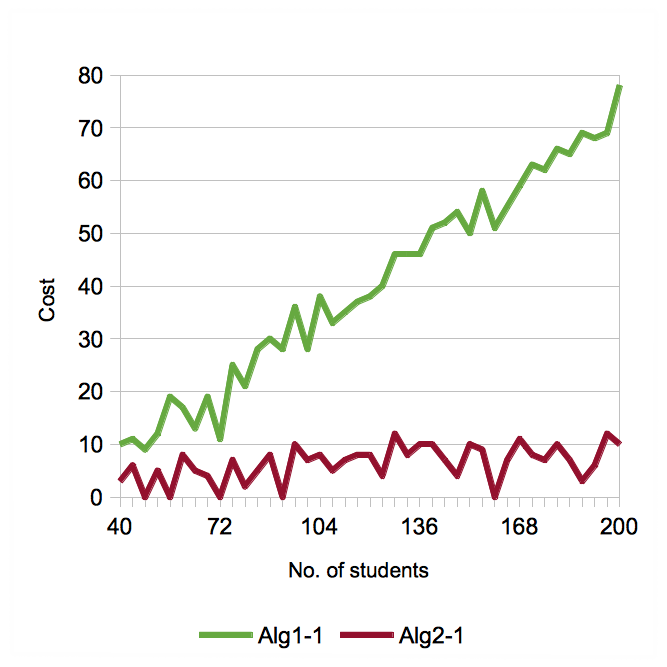
\includegraphics[width=0.45\textwidth]{slides/images/rand-01.png}
		}
		\hfill
		\subfloat[192 processes, $T_{0}=1.0$]{
			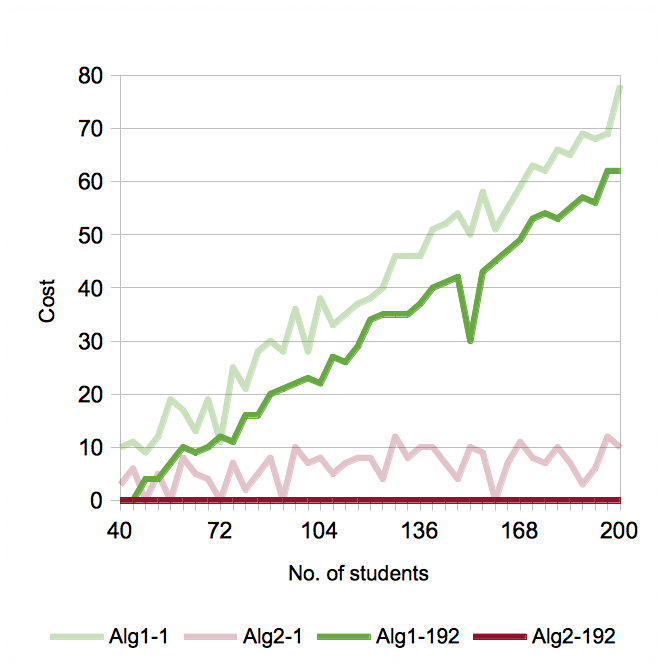
\includegraphics[width=0.45\textwidth]{slides/images/rand-192.png}
		}
		\hfill
		\ 
	\end{figure}
\end{frame}

\subsection{Initial temperature}
\begin{frame}
	\frametitle{Initial temperature}
	\begin{figure}[h]
		\centering
		\captionsetup[subfloat]{position=top}
		\hfill
		% \subfloat[\smaller 1 process, $T_{0}=\{\;1.0\;,\;10.0\;,\;10^{4}\;\}$]{
		\subfloat[Complete]{
			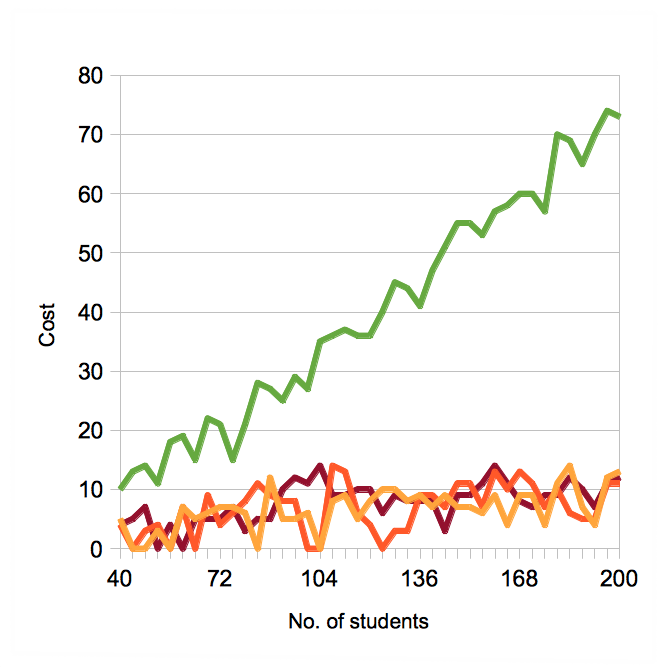
\includegraphics[width=0.45\textwidth]{slides/images/temp-cost.png}
		}
		\hfill
		% \subfloat[\smaller 1 process, $T_{0}=\{\;1.0\;,\;10.0\;,\;10^{4}\;\}$]{
		\subfloat[$10^{4}$ iterations]{
			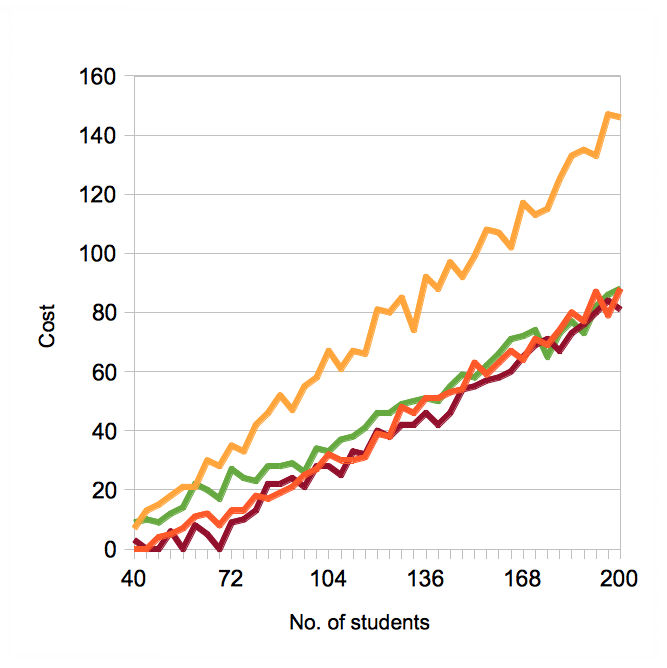
\includegraphics[width=0.45\textwidth]{slides/images/temp-cost-lim.png}
		}
		\hfill
		\ 

		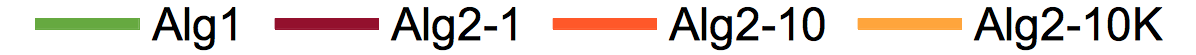
\includegraphics[width=0.6\textwidth]{slides/images/temp-leg.png}
	\end{figure}
\end{frame}